\documentclass{article}

% if you need to pass options to natbib, use, e.g.:
\PassOptionsToPackage{numbers, compress}{natbib}
% before loading nips_2018

% ready for submission
\usepackage[final]{nips_2018}
\usepackage{float}

% to compile a preprint version, e.g., for submission to arXiv, add
% add the [preprint] option:
% \usepackage[preprint]{nips_2018}

% to compile a camera-ready version, add the [final] option, e.g.:
% \usepackage[final]{nips_2018}

% to avoid loading the natbib package, add option nonatbib:
% \usepackage[nonatbib]{nips_2018}

\usepackage[utf8]{inputenc} % allow utf-8 input
\usepackage[T1]{fontenc}    % use 8-bit T1 fonts
\usepackage{hyperref}       % hyperlinks
\usepackage{url}            % simple URL typesetting
\usepackage{booktabs}       % professional-quality tables
\usepackage{amsfonts}       % blackboard math symbols
\usepackage{nicefrac}       % compact symbols for 1/2, etc.
\usepackage{microtype}      % microtypography
\usepackage{graphicx}

\title{How Are You Feeling? \\ Inferring Mood from Audio Samples}


% The \author macro works with any number of authors. There are two
% commands used to separate the names and addresses of multiple
% authors: \And and \AND.
%
% Using \And between authors leaves it to LaTeX to determine where to
% break the lines. Using \AND forces a line break at that point. So,
% if LaTeX puts 3 of 4 authors names on the first line, and the last
% on the second line, try using \AND instead of \And before the third
% author name.

\author{
  Joel Haynie \\
  Department of Computer Sciences\\
  University of Wisconsin, Madison\\
  \texttt{jhaynie@wisc.edu} \\
  \And
  Ankit Vij \\
  Department of Computer Sciences\\
  University of Wisconsin, Madison\\
  \texttt{vij2@wisc.edu} \\
  \AND
  Amanpreet Singh Saini \\
  Department of Computer Sciences\\
  University of Wisconsin, Madison\\
  \texttt{saini5@wisc.edu} \\
  \And
  Eric Brandt \\
  Department of Computer Sciences\\
  University of Wisconsin, Madison\\
  \texttt{ebrandt@wisc.edu}
}

\begin{document}
% \nipsfinalcopy is no longer used

\maketitle

\begin{abstract}
Classification of audio samples is an application of deep learning that is receiving considerable attention today. Our project involves investigating this specialized area of machine learning in detail. First, we explore the background and theoretical basis for audio sample classification using deep learning methods. Second, we implement and train a practical proof-of-concept application that classifies musical samples into one of four ‘moods’ and report test. Finally, we comment on emerging research topics in audio classification using deep neural networks.
\end{abstract}

\section{Motivation and Theoretical Basis}\label{sec:theory}

Our goal for this paper was to answer the following question, \textit{How does state-of-the-art audio clip based Machine Learning (ML) categorize the emotion / feeling of a song?}   Our research began by reading Hershey et al. \cite{hershey} influential paper on large scale audio classification.  This paper proposes using a Convolutional Neural Network (CNN) to aid in the classification.  The data flow from this paper can be seen in figure \ref{fig:vgg_flow}.  Our diagram was derived from the supplied code as the paper did not fully describe the data flow.  We can see that the flow is broken up into two key parts the preprocessing, via spectrographs, and the feature building, via CNN. 

\begin{figure}[!htb]
	\centering
	\includegraphics[width=1.0\textwidth]{VGG Flow.png}  
	\caption{Hershey et al. \cite{hershey} model of converting \texttt{.wav} audio to features suitable for ML}
	\label{fig:vgg_flow}
\end{figure}

As we continued to look for research, we found differing opinions within the ML community concerning the suitability of CNNs for audio-based training data.  A key dissent was written in a series of articles by Rothmann \cite{rothmann}, where he postulates that the present use of CNNs to do audio classification is insufficient and inaccurate.  He proposes a solution pictured in figure \ref{fig:rothman_flow}.   This data flow, he argues, more closely maps to the human ear.  

\begin{figure}[!htb]
	\centering
	\includegraphics[width=1.0\textwidth]{Rothmann_Flow.png}  
	\caption{Rothmann's	\cite{rothmann} ML model of human hearing}
	\label{fig:rothman_flow}
\end{figure}

Upon reading the works and looking closely at the two diagrams we see that the two approaches are nearly equivalent.  The GammaTone Filterbank and Dilated Circular Buffer proposed in \cite{rothmann}, are equivalent to well configured spectrographs from \cite{hershey}. More detail about \textit{well-configured} spectrographs can be read in section \ref{sec:preprocessing} Preprocessing below.  

In both approaches the preprocessed frequency domain data is fed into a learned model that reduces to a feature space for later stage classification.  Hershey et al.\cite{hershey} uses a CNN as seen in figure \ref{fig:vggish_cnn} to do this feature reduction.  Rothman \cite{rothmann} proposes one half of an Long Short-Term Memory (LSTM) AutoEncoder.  This implies that the key functional differences are the structure of the network and how the models are trained, CNN versus LSTM AutoEncoder.

The Purpose of an LSTM AutoEncoder is to take a large input space, convert it to a smaller representative space in order to return an approximation of the original input space.  Success is measured by how closely the large input space matches the large output space.  Once this intermediate representation space is obtained one uses that smaller space as the feature space for feeding into the classifier. Observe that no labelled data is needed to train the network.
Training a CNN needs labelled data to train the network.

Finally as an alternate view from the above two strategies there may be no need for these preprocessing stages at all. Dörfler et al. \cite{dorfler} prove, and Gong et al, \cite{gong} demonstrate that the spectrographs themselves can be removed by well defined layers in the feature reducing CNN.

\subsection{Preprocessing}\label{sec:preprocessing}

There are two key pre-processing portions referenced in \cite{rothmann}: GammaTone Filterbank and Dilated Circular Buffer.  Let us discuss how these compare to the Spectrograph as built in Hershey et al. \cite{hershey}.

Let us start by comparing GammaTone Filter banks(GFCC) to the Mel-Frequency Cepstral Coefficients(MFCC) used in each spectrograph column.  Burgos \cite{burgos} studied this in depth and found that the The MFCC are typically the de facto standard for speaker recognition systems because of their high accuracy and low complexity; however they are not very robust at the presence of additive noise. The GFCC features in recent studies have shown very good robustness against noise and acoustic change.  He further shows that there is about twice the performance improvement of GFCC over MFCC for very low, < -30dB, SNR values. He also shows there is little measurable difference for sounds where the Signal-to-Noise Ratio (SNR) goes above -5dB to 100dB.  The SNR of music can vary widely, thus over the vast majority of the range these two strategies have comparable outcomes.

Now let us focus our attention on the Dilated Circular Buffer and the specific hyperparameters used to calculate the spectrographs.  Rothmann \cite{rothmann} states that the Goal of the Dilated Circular Buffer is to emulate the echoic memory of human hearing.  According to him echoic memory can be considered as a short buffer of immediate auditory impressions. He clarifies that the biological research shows the duration of memory can vary from as short as 250 ms to 4 seconds. The Circular Buffer is a historical view of the frequency spectra, this is the definition of a spectrograph with zero window overlap.
In order to bound the size of the input set to the LSTM, he chooses to make the buffer \textit{Dilated}.  This strategy averages adjacent historical values into summary GFCC spectrums.  His input size is large because the temporal window’s length he applies the GFCC on is 5ms.  The key spectrograph hyperparameters are a frame or window length of 25ms and a hop length of 10ms.  The window length defines the \textit{resolution} of the spectrum. That is the smallest frequency that can be binned.  This affects the quality of the vertical axis of the spectrograph.  The hop length however reuses data already used in previous spectrum calculations which has the effect of blurring or averaging events in the spectrum. This yields a similar effect as Dilation.  Finally, the spectrograph’s used in \cite{rothmann} are 0.96 second in duration.  This is right in line with a \textit{echoic memory} of the human ear.

\subsection{VGGish’s CNN}\label{sec:vggishscnn}

In Hershey et al.\cite{hershey} the CNN is used to reduce the large input space, 10 x 6.1k x 4 byte values down to a more manageable and concise 10 x 128 byte feature vector. The shape and meaning of the data that leaves the preprocessing portion is 10 examples of 2-D log-mel-spectrograms of 96 overlapping frames covering 64 mel-log frequency bands.  
The CNN’s structure can be seen in figure \ref{fig:vggish_cnn}.  Specifically, the CNN contains all convolutions of 3x3 filters with strides of 1 and max pooling operations with 2x2 filter with strides of 2. With this configuration, the CNN contains in sequence, a convolution layer of 64 filters, a max-pooling layer, another convolution layer with 128 filters, another max-pooling layer, two convolution layers with 256 filters each, another max-pooling layer, another two convolution layers with 512 filters each, a max-pooling layer, from which the output is flattened and fed into two fully connected layers with 4096 outputs each, sequentially, and finally the output goes into a fully connected layer (the embedding layer) with 128 output units.
The CNN produces an output of 10 examples of the activations of the 128-D embedding layer.  This embedding is the 10x128 element feature vectors that can now be fed into the final stage, the classifier.

\begin{figure}[!htb]
	\centering
	\includegraphics[width=1.0\textwidth]{vggish_cnn_3.png}  
	\caption{Deep network layers of the VGGish Convolutional Neural Network}
	\label{fig:vggish_cnn}
\end{figure}
	
\section{Practical Implementation}

\subsection{Data Acquisition and Extraction}

We collected our data from Google’s AudioSet \cite{audioset} which consists of an expanding ontology of 632 audio event classes and a collection of 2,084,320 human-labeled 10-second sound clips drawn from YouTube videos. The ontology is specified as a hierarchical graph of event categories, covering a wide range of human and animal sounds, musical instruments and genres, and common everyday environmental sounds. From the dataset, we focused on music mood samples and extracted data instances having labels of four mood classes- \textit{Happy}, \textit{Sad}, \textit{Angry}, and \textit{Scary}. The dataset selected was divided into two groups: training and evaluation. 

To form our data sets, we filtered two disjoint sets from the ontology: First, a set of 400 instances with our corresponding labels for training. Of these 400, we ensured we chose 100 entries of each mood classification. The second set contained 223 data points with ~56 instances per label which we used for evaluating our models. To avoid contamination, these 223 data instances were held aside during training and not introduced to the model until the evaluation stage. We created \texttt{.csv} files containing, for each instance, the YouTube video ID, start and stop times within the video, and the label associated with the instance. These \texttt{.csv}s were then used to run a batch processing script to download the audio samples in \texttt{.wav} format directly from their source (YouTube).

\subsection{Transformation to Features}
The next step in the application pipeline is to transform the raw \texttt{.wav} files into features that can be input into a classifier network. This is done via the process described above in sections \ref{sec:preprocessing} and \ref{sec:vggishscnn}, using an open source TensorFlow model called VGGish \cite{vggish}. We made initial attempts to implement this layer ourselves, but the training required for the CNN to achieve suitable results is beyond the computational capacity of our local workstations. In this instance, `to see further, we stood on the shoulders of giants \cite{newton}’ (in this case, Google) and used the pre-trained CNN model to feature-ize the \texttt{.wav} files. We converted each of our 400+223 \texttt{.wav} file instances using VGGish to 10x128 element feature vectors.

\subsection{Classification}

After initial processing of the wav files into feature vectors (matrices) of dimension 10x128 we investigated different models to perform the multi-class classification task of predicting the \textit{mood} of the music from the feature vector.

To evaluate different classification models, Python was used, enlisting the libraries TensorFlow \cite{tensorflow} and Keras \cite{keras}.

The 400 training samples were evenly divided by class for stratified cross validation and used to train 3 different neural networks:
\begin{enumerate}
\item Simple multi-class logistic regression classifier
\item 1-Layer LSTM (Long-short term memory) recurrent neural network
\item 3-Layer LSTM (Long-short term memory) recurrent neural network
\end{enumerate}
In each case, the model was trained using batches of 40 samples, randomized at each presentation, for a sufficient number of epochs to infer steady-state accuracy.

We evaluated the performance of each of the 3 models by two methods:
\begin{enumerate}
\item Validation set accuracy over an increasing number of epochs to watch for over-training and the any generalization gap.
\item Evaluation on our Test Set of 223 never-seen-before data instances.
\end{enumerate}

The performance of the training sessions is shown in figure \ref{fig:baseline_train}.
\begin{figure}[!htb]
	\centering
	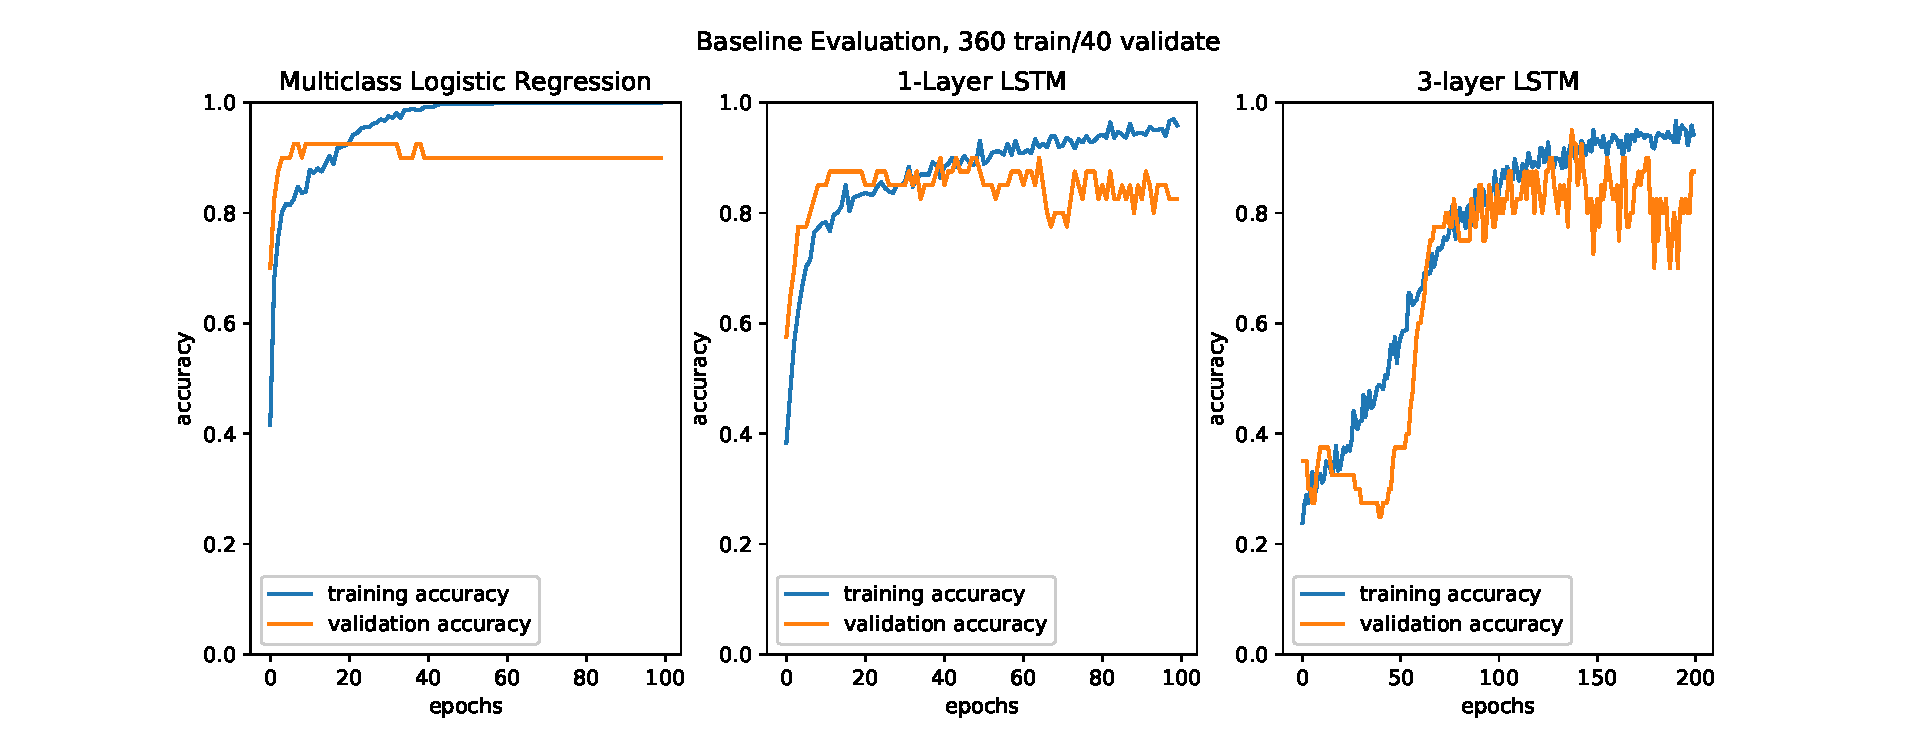
\includegraphics[width=1.0\textwidth]{Baseline400.eps}  
	\caption{Training performance for 3 models.}
	\label{fig:baseline_train}
\end{figure}

After training, the evaluation on the 223-instance test set, we observed the accuracies shown in table \ref{tbl:baseline_acc}.
\begin{table}[!htb] 
\caption{Accuracy on held-aside test set of 223 instances for 3 models.}
\label{tbl:baseline_acc}
\centering
\begin{tabular}{lc} 
\toprule
\hline
Model & Accuracy \\ 
\midrule
Logistic Regression & 0.798 \\
1-Layer LSTM & 0.839 \\ 
3-Layer LSTM & 0.776 \\ 
\bottomrule
\end{tabular}
\end{table}

Finally, to make sure that our four chosen classes do not have an abnormal correlation between any combinations of classes, we also computed confusion matrices for the models. The confusion matrix for 1-LSTM (arguably the best performing classifier) is shown in table \ref{tbl:baseline_conf}.

\begin{table}[!htb] 
\caption{Confusion matrix for 1-LSTM classifier of 223 test instances.}
\label{tbl:baseline_conf}
\centering
\begin{tabular}{lcccc} 
\toprule
\hline
 & Happy & Sad & Angry & Scary \\ 
\midrule
Happy & 45 &  9 & 2 & 1 \\
Sad   &  11 & 39 & 2 & 4 \\
Angry &  0 &  1 & 53 & 4 \\
Scary &  0 &  7 & 3 &  42 \\
\bottomrule
\end{tabular}
\end{table}

\section{Conclusion}

\subsection{Discussion}

After evaluating Logistic Regression, 1-Layer LSTM, and 3-Layer LSTM learning models on the evaluation set, we can draw some important conclusions. First, the input feature sets (output of VGGish) must already be nearly linearly separable, as evidenced by the strong performance of the simple multiclass logistic regression classifier. VGGish’s preprocessing of the raw audio waveforms into 10x128 element feature vectors clearly has produced data that is well separated without significant further processing. Evidence of the linearly separable feature data is supported by the fact that much more complicated non-linear classifiers (1-Layer LSTM and 3-Layer LSTM) do not yield better performance. Second, it is also clear that complicated models with more parameters, particularly the 3-Layer LSTM take significantly more time to train. There is evidence that the LSTM models are subject to overtraining at higher numbers of epochs, as validation set accuracy decreases somewhat with increasing number of epochs. This leads us to believe that for the practitioner who wishes to write an audio-based ML application and use AudioSet and VGGish as a `black box', he or she is likely to do very well with only a simple linear classifier at the end. Finally, specific to our data set, the confusion matrix suggests, surprisingly, that ‘Happy’ and ‘Sad’ are the most often confused classifications, and that ‘Scary’ and ‘Angry’ are comparatively easy to predict. 

\subsection{Future Work}

In the future, we plan to extend the capabilities and accuracy of our model and by including recent developments taking place in the field of sound recognition. Tokozume et al. \cite{tokozume} talk about Between-Class learning (BC learning) which is a novel learning method for deep sound recognition. In a similar direction to overcome undesirable behaviors such as memorization and sensitivity to adversarial examples by neural networks, Zhang et al. \cite{zhang} propose a simple learning principle called mixup. Both approaches train neural networks on convex \textit{combinations} of pairs of examples and their label. This creates a new feature space by combining sounds from different classes. This would not only provide variations in feature space and remove sensitivity to adversarial examples, but will also regularize the positional relationship between the class feature distributions. The results from the two papers also show that the model provides better performance, so exploring this direction could provide better accuracy in mood detection from audio. 

Another direction that is also very appealing is the use of speaker adaptation and regularization techniques for neural networks for sound recognition. Tomashenko et al. \cite{tomashenko} propose a novel way to improve speaker adaptive training for neural network acoustic models using GMM derived features for automatic speech recognition. Taking inspiration from this work, we can also extend our system to detect mood from user’s speech using the techniques as suggested by Tomashenko et al. which will improve its capabilities of mood detection beyond music. 

As a future application, the detection of mood from audio signals could be put to use for various recommendation systems. One possible application is the mood based song recommendation service and another could be targeted product recommendation based on inferred mood of the listener. There could be other possible applications like depression detection systems based on the user’s choice of audio playlists etc.  
  
\bibliography{Bibliography} 
\bibliographystyle{plainnat}

\end{document}


